\chapter{Koncepcja powiązania analizy sentymentu i geolokacji w badaniu
zachowań użytkowników sieci społecznościowych.}

W tym rozdziale opisany jest sposób realizacji celów mojej pracy magisterskiej
-- czyli sposób powiązania ze sobą analizy sentymentu i geolokacji w kontekście
badania zachowań użytkowników sieci społecznościowych. W podrozdziale
\ref{section:modelsystemu} zaprezentowany został model systemu z uwzględnieniem
przetwarzania wstępnego \ref{subsection:zbieraniedanych}, modelu analizy
sentymentu \ref{subsection:modelanalizysentymentu}, modelu grup społecznych
\ref{subsection:modelgrupirelacjispolecznych} i modelu geolokacji
\ref{subsection:modelgeolokacji}. Następnie przedstawione są wielkości
wykorzystywane w eskperymentach \ref{section:wielkosciwykorzystywane}, a na
końcu szczegółowo została opisana koncepcja i algorytm analizy sentymentu
\ref{section:koncepcjaialgorytmanalizysentymentu}.



% =============================================================================
\section{Model systemu}
\label{section:modelsystemu}
% =============================================================================
Ogólny model systemu został przedstawiony na rysunku \ref{image:model-systemu}.

\begin{figure}[ht!]
\centering
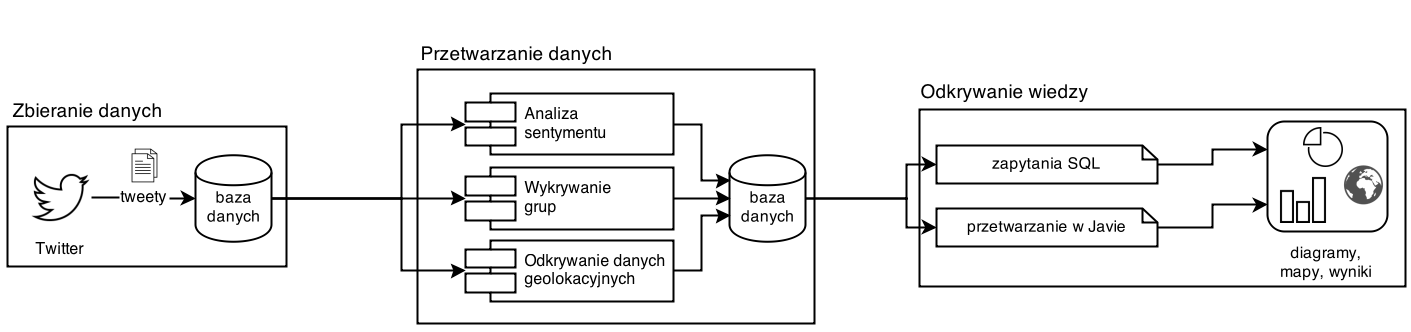
\includegraphics[width=160mm]{img/gruby-model.png}
\caption{Ogólny model systemu}
\label{image:model-systemu}
\end{figure}


Można go podzielić na trzy następujące części (podpisane na wspomnianym
rysunku):
\begin{enumerate}
  \item Zbieranie danych.
  \item Przetwarzanie i uzupełnianie danych.
  \item Zdobywanie wiedzy z zebranych i przetworzonych danych.
\end{enumerate}



\clearpage
\subsection{Zbieranie danych}
\label{subsection:zbieraniedanych}
Zbieranie danych jest pierwszym elementem składowym całego systemu.
Jego koncepcje przedstawia rysunek \ref{image:zbieranie-danych}.
Jest to bardzo ważny składnik systemu. Aby móc przeprowadzić jakiekolwiek
analizy potrzeba najpierw zebrać dane.

\begin{figure}[ht!]
\centering
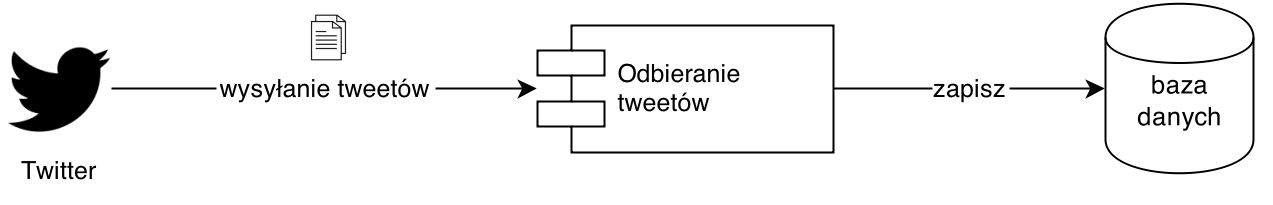
\includegraphics[width=160mm]{img/zbieranie-danych.png}
\caption{Zbieranie danych}
\label{image:zbieranie-danych}
\end{figure}


Zbieranie danych z serwisu Twitter odbyło się przy pomocy wspomnianego w sekcji
\ref{subsection:twitterjakozrodlodanych} Twitter Streaming API. Napisany został
program w Javie, który nasłuchiwał w trakcie każdego śledzonego meczu wpisów w
języku angielskim, które zawierały odpowiednie słowa kluczowe. Były nimi
przygotowane wcześniej słowa związane z danym spotkaniem: nazwiska i przydomki
piłkarzy, menadżerów, nazwy i przydomki klubów, nazwa stadionu czy nazwisko
sędziego. W taki sposób uzyskiwano tweety, które można było powiązać z
konkretnym meczem.

Program do nasłuchiwania uruchamiany jest na czas trwania meczu z pewnym
marginesem przed i po spotkaniu. Jest to o tyle ważne, że udostępnione API służy
tylko do konsumowania wpisów na żywo. Pobranie tych samych wpisów już po danym
wydarzeniu byłoby dużo bardziej skomplikowane. Program otrzymuje nie więcej niż
1\% wszystkich wpisów w danym momencie na Twitterze \footnote{Jeśli w danym
momencie na Twitterze jest 1000 wpisów, z czego 10 z podanymi słowami
kluczowymi, wówczas program otrzyma wszystkie 10 wpisów. Jeśli z określonymi
słowami kluczowymi byłoby więcej wpisów, wówczas program nadal otrzymałby tylko
10 z nich.}. Każdemu wpisowi nadawany jest identyfikator meczu (wprowadzonego
wcześniej do bazy danych) i w takiej postaci jest on zapisywany do bazy.

W ten sposób zbieranie są dane z Twittera. Podejście to pozwala na elastyczną
wymianę słów kluczowych do nasłuchiwania, gdyż program na wejściu potrzebuje
jedynie identyfikator meczu, do którego już są przypisane słowa kluczowe.




\subsection{Model analizy sentymentu}
\label{subsection:modelanalizysentymentu}

Analiza sentymentu należy do jednego z elementów drugiej części systemu.
W tej części zebrane uprzednio dane były przetwarzane, między innymi pod kątem
oceny ich sentymentu. Proces ten przebiegał według schematu
zaprezentowanego na rysunku \ref{image:model-analizy-sentymentu}.

\begin{figure}[ht!]
\centering
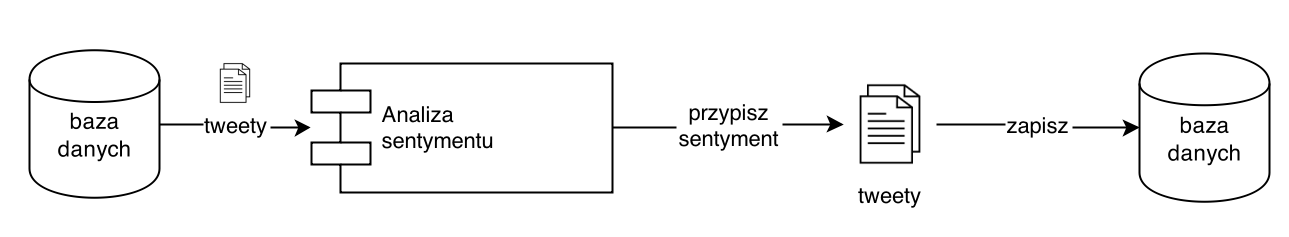
\includegraphics[width=160mm]{img/model-analizy-sentymentu.png}
\caption{Model analizy sentymentu}
\label{image:model-analizy-sentymentu}
\end{figure}


Dla każego tweeta w bazie obliczana była jego wartość \textit{valence}.
Aby do tego doszło tweet był wcześniej odpowiednio oczyszczany z wszystkich
elementów, które mogły zakłócić wyliczenie tej wartości. Proces przebiegał
zgodnie z pomysłem i algorytmem panów Pak i Paroubek (krótko omówiony w sekcji
\ref{subsubsection:pakandparoubek}), a szczegóły jego działania wraz z
zastosowaną przez ze mnie modyfikacją (polegającą na dodaniu wykrywania negacji)
zostały opisany w sekcji \ref{section:koncepcjaialgorytmanalizysentymentu}.

Po wyliczeniu wartości \textit{valence} dla zebranych tweetów obliczona została
jego średnia wartość i wpisy o wartości wyższej od średniej zostały oznaczone
jako pozytywne, zaś o wartości niższej jako negatywne (zgodnie z pomysłem Paka
i Paroubeka).

Oznaczenie wartości sentymentu zebranych wpisów pozwoliło na przeprowadzenie
ciekawych eksperymentów opisanych w rozdziale \ref{chapter:eksperymenty}.


\subsection{Model grup i relacji społecznych}
\label{subsection:modelgrupirelacjispolecznych}



\begin{figure}[ht!]
\centering
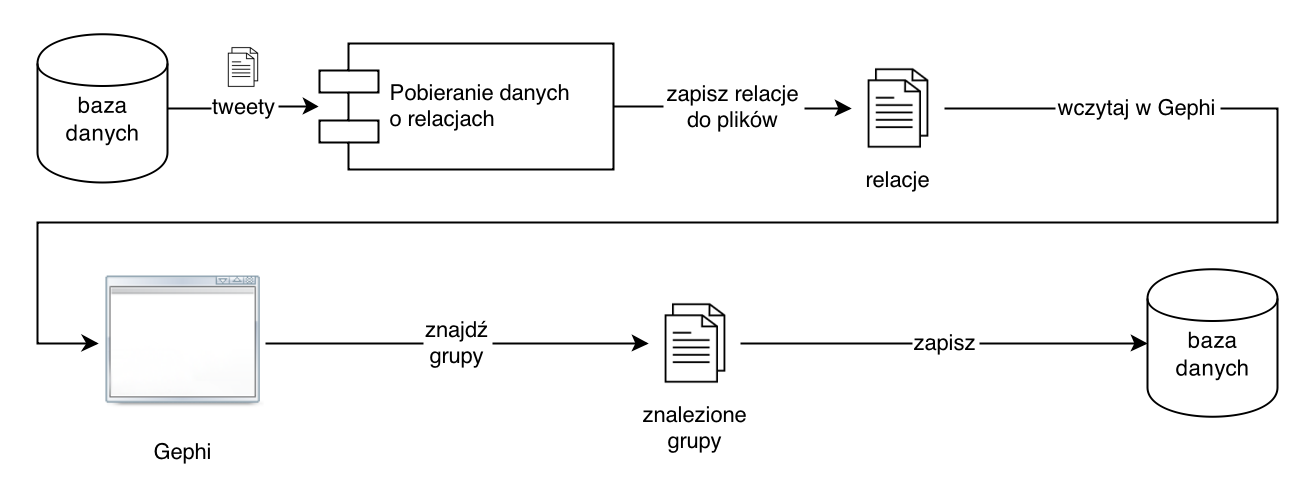
\includegraphics[width=160mm]{img/odkrywanie-relacji.png}
\caption{Model grup i relacji społecznych}
\label{image:odkrywanie-relacji}
\end{figure}

\subsection{Model geolokacji}
\label{subsection:modelgeolokacji}



\begin{figure}[ht!]
\centering
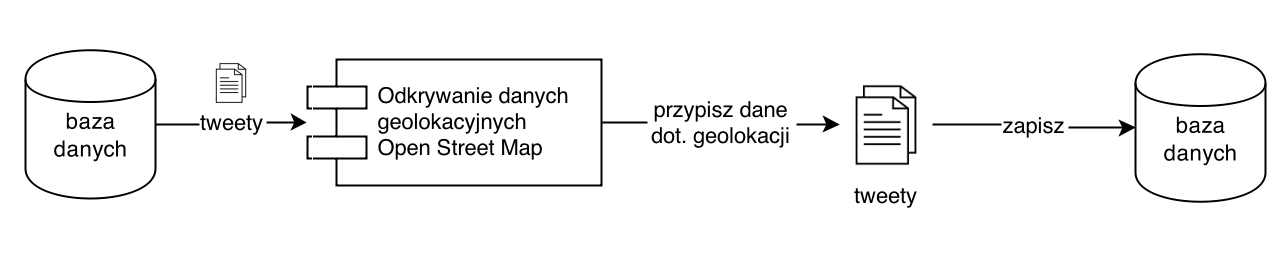
\includegraphics[width=160mm]{img/odkrywanie-geolokacji.png}
\caption{Model geolokacji}
\label{image:odkrywanie-geolokacji}
\end{figure}





% ==============================================================================
\section{Wielkości i techniki wykorzystywane w eksperymentach}
\label{section:wielkosciwykorzystywane}
% ==============================================================================
\subsection{Analiza sentymentu}
\subsubsection{Ocena pozytywności wpisu}
\label{subsection:ocenapozytywnosci}
W kilku miejscach została zastosowana miara pozytywności wpisu.
Została ona wyliczona przy pomocy następującego równania:

\begin{equation}
\label{equation:pozytywnosc}
P = \frac{|pos|}{|pos| + |neg|}
\end{equation}

gdzie:

$|pos|$ -- liczba wpisów oznaczonych jako pozytywne,

$|neg|$ -- liczba wpisów oznaczonych jako negatywne.



\subsubsection{Wykrywanie zwolenników i przeciwników klubu}
\label{subsubsection:wykrywaniezwolennikow}

Proces oznaczania użytkowników jako sympatyków i przeciwników drużyny przebiegał
w następujący sposób:
\begin{itemize}
  \item dla każdego użytkownika zliczono jego wpisy w meczach każdej z badanych 
  drużyn,
  \item jeśli w meczach drużyny A dla danego użytkownika przeważała liczba 
  wpisów pozytywnych, wówczas oznaczano takiego kibica jako zwolennika drużyny A,
  \item jeśli natomiast przeważała liczba wpisów negatywnych, wówczas taki kibic
  traktowany był jako przeciwnik danej drużyny.  
\end{itemize} 

\subsection{Relacje}



\subsubsection{Wykrywanie grup}
 \label{subsubsection:koncepcja-wykrywaniegrup}
% gephi, modularity
Do wykrywania grup wśród sieci społecznych skorzystałem z narzędzia
otwartoźródłowego narzędzia \textit{Gephi} wspomagającego analizę grafową, w
którym został zaimplementowany algorytm przedstawiony w artykule
\cite{blondel2008fuc}. Przy jego użyciu konkretne węzły zostały podzielone
na grupy, nad którymi przeprowadzałem późniejsze analizy.

Grupy zostały zbudowane na podstawie relacji \textit{reply}
stworzonej z zebranych wpisów. Na podstawie odpowiedzi między różnymi
użytkownikami budowany był model sieci społecznej.
W każdym kolejnym meczu przeprowadzono badanie grup wśród użytkowników.
Uzyskane wyniki podzielono na trzy ,,koszyki''. W pierwszym znalazły się grupy 
3 lub 4 osobowe. W~drugim koszyku grupy mające od 5 do 9 osób, a w trzecim koszyku
większe grupy. 


\subsubsection{Badanie podobieństwa grup}
\label{subsection:badaniepodobienstwagrup}
Badanie podobieństwa oparte było o analizę kolejnych wydarzeń. 
Polegało na zliczeniu ile wierzchołków powtarza się w kolejnych meczach.
Oparte zostało o niniejsze równanie:
\begin{equation}
S = \frac{|V_1 \cap V_2|}{|V_1|}
\end{equation}  
gdzie:

$V_1$ -- zbiór wierzchołków w pierwszym wydarzeniu,

$V_2$ -- zbiór wierzchołków w drugim wydarzeniu.

Krótko mówiąc podobieństwo to iloraz liczby wspólnych wierzchołków między 
wydarzeniami a liczby wierzchołków w pierwszym z nich.








\subsection{Geolokacja}
\subsubsection{Badanie odległości między użytkownikami}
\label{subsubsection:badanieodleglosci}
TODO napisać trochę więcej.

Badanie odległosci między użytkownikami odbyło się na podstawie odpowiedzi z
geolokacją -- retweety nie zawierają informacji o położeniu użytkownika.
Spośród tych użytkowników, którzy pisali z geolokacją zostało zliczone ilu z
nich się ze sobą komunikowało w zależności od wzajemnej odległości.






\subsubsection{Badanie odległości od stadionu}
\label{subsubsection:badanieodleglosciodstadionu}
TODO opisać 














% ==============================================================================
\section{Koncepcja i algorytm analizy sentymentu}
\label{section:koncepcjaialgorytmanalizysentymentu}
% ==============================================================================

W tym miejscu opisuję sposób w jaki została użyta do moich badań analiza
wydźwięku wypowiedzi. Przedstawiam czynności wstępne jakie zostały zastosowane
na tekście, prezentuję krótko wybrany algorytm i zastosowane w nim modyfikacje
oraz opisuję sposób zaaplikowania analizy wydźwięku na zgromadzonych tweetach.

\subsection{Normalizacja tekstu}
\label{subsection:normalizacjatekstu}
% pozbycie się słów kluczowych, zaprzeczenia, retweety

W związku z tym, że wpisy są tworzone przez zwykłych użytkowników posiadają one
wiele znaków i elementów, które z punktu widzenia analizy sentymentu są zbędne,
a czasami prowadzące do błędów. Dlatego też tekst należy poddać normalizacji,
usunięciu zbędnych elementów, szumów i spamu. Przykładowa lista wpisów jakie
znalazły się w zgromadzonych danych przedstawia poniższa tabela
(\ref{tab:wpisy-przed-normalizacja}).


\begin{table}[ht!]  
\begin{center}  
\begin{tabular}{|r|p{140mm}|}
\hline
\multicolumn{2}{|c|}{Przed normalizacją}
\\ \hline
1 & RT @J\_SPEKZ: Haha quality! \#Fellaini \#United \#Moyes
http://t.co/rJB4K1fvZy
\\ \hline
2 & Stay woke brah! The Arsenal is about to make everything alright soon :) RT
@JCphoenixx: So damn tired, So not sleepy.
\\ \hline
3 & @abdul1haseeb My arsenal is not disappointing too :P 
\\ \hline
4 & @Arsenal didn't think i could respect @aaronramsey any more than i already
did, bute what a gentleman he is for not to celebrate that goal:) 
\\ \hline
5 & OHHHHHH!!!!! SO CLOSE!!! Wilshere!!! Good Job Ramsey keeping that move alive
\\ \hline
6 & Haha, you gotta agree, no one gets booed like Manchester United :D \#ZeDevilza
\\
\hline
\end{tabular} 
\end{center} 
\caption{Przykładowa lista wpisów przed normalizacją}
\label{tab:wpisy-przed-normalizacja}
\end{table}


Po przeprowadzeniu wszystkich prac związanych z normalizacją tekstu wpisy z
powyższej tabeli prezentują się w następujący sposób:

\begin{table}[ht!]  
\begin{center}  
\begin{tabular}{|r|p{140mm}|}
\hline
\multicolumn{2}{|c|}{Po normalizacji}
\\ \hline
1 & 
\\ \hline
2 & stay woke brah make alright
\\ \hline
3 & not\_disappointing
\\ \hline
4 & didnt not\_respect bute gentleman not\_celebrate not\_goal
\\ \hline
5 & ohhhhhh close good job keeping alive
\\ \hline
6 & haha gotta agree not\_booed
\\
\hline
\end{tabular} 
\end{center} 
\caption{Lista wpisów poddanych normalizacji}
\label{tab:wpisy-po-normalizacja}
\end{table}

Kolejne kroki, które przekształciły tweety do powyższej postaci to:
\begin{enumerate}
  \item Usunięcie skomentowanych retweetów.\\
  \texttt{Stay woke brah! The Arsenal is about to make everything
  alright soon :) \sout{RT @JCphoenixx: So damn tired, So not sleepy.}}
  
  \item Usunięcie skomentowanych cytowań. \\
  \texttt{At all...\sout{"@dotun\_somoye: Even city's first goal
  negredo was offside....:( the refs not helping at all"} }
  
  \item Usunięcie hiperlinków.\\
  \texttt{You up for Arsenal's match later on? - what time? maybe if i'm not
  busy baby sitting :) \sout{http://t.co/aC5Ec8ipy1}}
 
  
  \item Usunięcie nazw użytkowników.\\
  \texttt{\sout{@abdul1haseeb} My arsenal is not disappointing too :P}
  
  
  \item Usunięcie hashtagów. \\
  \texttt{Haha, you gotta agree, no one gets booed like Manchester United :D
  \sout{\#ZeDevilza}}
  
  
  \item Oznaczenie wyrazów zaprzeczonych przedrostkiem \texttt{NOT\_} (opisuję
  dokładniej w sekcji \ref{subsection:sentyment-algorytm}). \\
  \texttt{didn't \textbf{NOT\_think NOT\_i NOT\_could NOT\_respect NOT\_any 
  NOT\_more NOT\_than NOT\_i NOT\_already NOT\_did}, bute what a gentleman he 
  is for not \textbf{NOT\_to NOT\_celebrate NOT\_that NOT\_goal:)}}

 \item Zachowanie tylko znaków alfabetu:
  	\begin{itemize}
  		\item usunięcie zaimków dzierżawczych (\texttt{Helen's} $\to$ \texttt{Helen}),
  		\item usunięcie apostrofu ze skróconych zaprzeczeń (\texttt{don't} $\to$ \texttt{dont}),
  		\item normalizacja liter diakrytyzowanych (\texttt{José Mourinho} $\to$ \texttt{Jose
  		Mourinho})
  		\item usunięcie liczb i wszelkich znaków niealfabetycznych.
	\end{itemize}

  \texttt{You up for Arsenal\sout{'s} match later on\sout{? -} what
  time\sout{?} maybe if i\sout{'}m not busy baby sitting \sout{:)}} 
	
	\item Usunięcie wyrazów zdefiniowanych w stop liście (powszechne wyrazy danego
	języka, które mogą być pominięte nie tracąc jednocześnie żadnej informacji).
	Zastosowałem stop listę z serwisu \mbox{WebPageAnalyse.com} 
	\cite{WebPageAnalyse} zawierającą 528 słów.

	\texttt{\sout{You up for} Arsenal match \sout{later on what} time \sout{maybe if} 
 	im \sout{not} busy baby sitting}
	
	\item Usunięcie słów kluczowych, które użyte były do gromadzenia wpisów z
	Twittera -- czyli nazwisk piłkarzy, menadżerów, nazw klubów, itd.
	
	%\texttt{\sout{BENDTNER} FUCKING im \sout{NOT\_arsenal} NOT\_fan}
	
	\texttt{OHHHHHH CLOSE \sout{Wilshere} Good Job \sout{Ramsey} keeping alive}
	
\end{enumerate}





\subsection{Zastosowanie algorytmu}
\label{subsection:sentyment-algorytm}
% + dobór parametrów, emotikony, zaprzeczenia

Do przeprowadzenia analizy sentymentu na zebranych tweetach skorzystałem z
metody opracowanej przez Alexandra Paka i Patricka Paroubek'a, którą krótko
przedstawiłem w sekcji \ref{subsubsection:pakandparoubek}.
Jest to technika, która pozwala badać sentyment nie posiadając wcześniej
słownika sentymentu. Dlatego też pierwszym krokiem jest zbudowanie takiego
słownika z zebranych danych.
W tym celu wybiera się podzbiór wpisów, które zawierają emotikony.
W związku ze 140 znakowym ograniczeniem na długość znaków przyjmuje się
założenie, że dana emotikona nadaje wydźwięk całemu wpisowi.
Według artykułu \cite{EmoticonAnalysisTwitter} 20 emotikon pokrywa w 90\%
stosowanie tych znaków graficznych we wpisach (na 100 wpisów z emotikonami, 90 z
nich zawiera emotikonę ze zbioru tych 20). Dlatego też skorzystałem z tego
zbioru do własnych badań dzieląc emotikony na wyrażające wydźwięk pozytywny i
negatywny w sposób\footnote{emotikona \texttt{D:} została pominięta, gdyż
pokrywała więcej przypadków niż tylko użycie emotikony (np.:
\texttt{Accepte\textbf{d:} Mary, John, Jane})} przedstawiony w tabeli
\ref{tab:wydzwiek-emotikon}.

\begin{table}[ht!]  
\begin{center}  
\begin{tabular}{|c|r|l|}
\hline
Emotikona & Popularnoś według \cite{EmoticonAnalysisTwitter} &
Wydźwięk \\ \hline
\texttt{:)} & $33.4\%$ & pozytywny \\ \hline
\texttt{:D} & $11.0\%$ & pozytywny \\ \hline
\texttt{:(} & $7.9\%$ & negatywny \\ \hline
\texttt{;)} & $7.5\%$ & pozytywny \\ \hline
\texttt{:-)} & $4.4\%$ & pozytywny \\ \hline
\texttt{:P} & $3.7\%$ & pozytywny \\ \hline
\texttt{=)} & $3.7\%$ & pozytywny \\ \hline
\texttt{(:} & $2.8\%$ & pozytywny \\ \hline
\texttt{;-)} & $2.2\%$ & pozytywny \\ \hline
\texttt{:/} & $1.9\%$ & negatywny \\ \hline
\texttt{XD} & $1.9\%$ & pozytywny \\ \hline
\texttt{=D} & $1.5\%$ & pozytywny \\ \hline
\texttt{:O} & $1.1\%$ & pozytywny \\ \hline
\texttt{=]} & $1.1\%$ & pozytywny \\ \hline
\texttt{;D} & $1.0\%$ & pozytywny \\ \hline
\texttt{:]} & $1.0\%$ & pozytywny \\ \hline
\texttt{:-(} & $0.8\%$ & negatywny \\ \hline
\texttt{=/} & $0.8\%$ & negatywny \\ \hline
\texttt{=(} & $0.8\%$ & negatywny \\ \hline
\end{tabular} 
\end{center} 
\caption{Wydźwięk emotikon}
\label{tab:wydzwiek-emotikon}
\end{table}

Następnie przeglądnięto wszystkie tweety z emotikonami zliczając liczbę
występowania wyrazów w kontekście pozytywnym i negatywnym.
Najpierw badano sentyment całego wpisu (na podstawie emotikony -- gdy była ich
większa ilość wybierano ten sentyment, który przeważał) a następnie dla każdego
wyrazu z tego wpisu zwiększano licznik odpowiednio wystąpień pozytywnych lub
negatywnych. Oczywiście wpisy były już poddane normalizacji.
W ten sposób uzyskano słownik sentymentu zbudowany z zebranych danych, który
zawierał 34183 słowa, a najpopularniejsze z nich zaprezentowane są w tabeli
\ref{tab:liczebnosc-slow-sentymentu}, gdzie:

wartość \textit{valence} wyliczna jest według wzoru \ref{equation:pakparoubek} 
i używana jest w dalszych obliczeniach,

wartość pozytywności wyliczona jest według wzoru \ref{equation:pozytywnosc}.

\begin{table}[ht!]  
\begin{center}  
\begin{tabular}{|l|r|r|r|r|}
\hline
Słowo & Wyst. pozytywne  & Wyst. negatywne 
& Pozytywność
& Valence
\\ \hline 
win & 4206 & 598 & 87.6 \% & 0.845 \\ \hline
good & 3916 & 435 & 90.0 \% & 0.903 \\ \hline
game & 3016 & 1012 & 74.9 \% & 0.301 \\ \hline
goal & 2305 & 584 & 79.8 \% & 0.477 \\ \hline
today & 2019 & 526 & 79.3 \% & 0.477 \\ \hline
time & 1844 & 404 & 82.0 \% & 0.602 \\ \hline
dont & 1461 & 775 & 65.3 \% & 0.000 \\ \hline
match & 1669 & 449 & 78.8 \% & 0.477 \\ \hline
great & 1885 & 160 & 92.2 \% & 1.041 \\ \hline
love & 1837 & 202 & 90.1 \% & 0.954 \\ \hline
\end{tabular} 
\end{center} 
\caption{Liczba występowania najpopularniejszych słów w zbudowanych słowniku
sentymentu}
\label{tab:liczebnosc-slow-sentymentu}
\end{table}

Dla każdego wpisu wyliczana jest średnia arytmetyczna wartości \textit{valence}
wszystkich słów. W ten sposób wylicza sie wartość \textit{valence} danego wpisu.
W tabeli \ref{tab:valence-przyklad} prezentuję przykładowe wyniki wyliczania tej
wielkości.

\begin{table}[ht!]
\begin{center}  
\begin{tabular}{|p{12mm}|p{70mm}|>{\raggedright\arraybackslash}p{60mm}|}
\hline
Valence & Wpis & Składowe 
\\ \hline 
0.6261 POS & Just seen you in the crowd at Chelsea game! @domashman http://t.co/NjovoZdgZ3 & {game=0.4740, crowd=0.7782}
\\ \hline
0.5909 POS & RT @BTSP: \#PRIZEDRAW If Arsenal win tonight one lucky person
will win a personalised BTSP mug! Simply RT \& follow to enter!
http://t.co/9m... & {lucky=0.4613, tonight=0.6873, btsp=0.3010, person=0.4232, personalised=0.3010, enter=0.5351, follow=1.2229, win=0.8465, mug=0.4771, simply=0.3979}
\\ \hline
0.6199 POS & Liking the brightness of this Napoli kit \#tempted &
{liking=0.8062, kit=0.4337} \\ \hline
0.0305 NEG & @ricktaylor1987 You're not watching Arsenal? &
{not\_watching=0.0305} \\ \hline
0.1234 NEG & Poor start\#AFC & {poor=-0.2848, start=0.5317}
\\ \hline
0.1807 NEG & Do Arsenal have any players who don't fall down with ease?
\#SwimmingTeam & {players=0.3684, not\_fall=-0.3979, not\_ease=0.4771,
dont=0.2751} \\ \hline
\end{tabular} 
\end{center} 
\caption{Wynik działania algorytmu analizy sentymentu na przykładowych wpisach}
\label{tab:valence-przyklad}
\end{table}

Określenie sentymentu wpisu odbywa się zgodnie z równaniem:
\begin{equation}
S(t) =
\begin{cases}
POS & valence(t) > AVG\_VALENCE \\
NEG & valence(t) <= AVG\_VALENCE \\
\end{cases}
\end{equation}

gdzie:

$AVG\_VALENCE$ jest średnią arytmetyczną wartości $valence$
wszystkich wpisów. W moich badaniach wartość ta wyniosła $0.4786984978198536$.

\subsubsection{Wykrywanie i obsługa negacji}
\label{subsubsection:wykrywanieiobsluganegacji}
W oryginalnym podejściu panów Pak i Paroubek nie ma żadnego sposobu na
wykrywanie i obsługę negacji. Oczywistym jednak jest, iż zaprzeczenia zmieniają
znaczenie dalszej części tekstu i muszą być w jakiś sposób obsłużone.
Wpisy na Twitterze są krótkie, więc postanowiłem zastosować podejście
zaprezentowane w artykule \cite{thumbsUp2002}, które polega na dodaniu
przedrostka \texttt{NOT\_} do wszystkich słów pomiędzy wyrazem negującym,
a najbliższym znakiem przestankowym. Lista wyrazów negujących
została zaczerpnięta z \cite{englishNots1983}. Słowa zanegowane miały osobno
liczone liczby wystąpień w kontekstach pozytwnych i negatywnych. W takiej formie
brały udział w ocenie sentymentu wpisów z Twittera.







\subsubsection{Dobór parametrów}
\label{subsubsection:doborparametrow}
Użyty przeze mnie algorytm zakłada dobór parametrów przed przeprowadzeniem
analizy sentymentu. Parametry te dotyczą słów ze zbudowanego słownika --
decydując, które z nich wezmą udział w procesie analizy. Są to: minimalna
długość słowa, minimalna liczba występowania słowa. Doboru parametrów dokonałem
w sposób zaprezentowany w opisie algorytmu. Wykorzystałem listę wpisów z
emotikonami, podzieliłem je na zbiór uczący i testowy w stosunku 20\% do 80\%.
Wygenerowałem słownik ze zbioru uczącego. Wpisy ze zbioru testowego oznaczyłem spodziewanym
sentymentem -- był to sentyment emotikony jaką zawierały. Następnie
przeprowadziłem testy poprawności klasyifkacji zbioru testowego słowami ze
zbioru uczącego dla wyrazów o minimalnej długości od 1 do 10 i minimalnej
liczbie wystąpień od 1 do 100 -- daje to w sumie 1000 testów.
Najwyższy stopień poprawności klasyfikacji uzyskałem dla parametrów równych:
minimalna długość wyrazu -- 3, \mbox{minimalna częstotliwość wystąpień -- 1}.
Wyniki testów przedstawiam na poniższym wykresie
\ref{image:pak-paroubek-parametry}.

\begin{figure}[ht!]
\centering
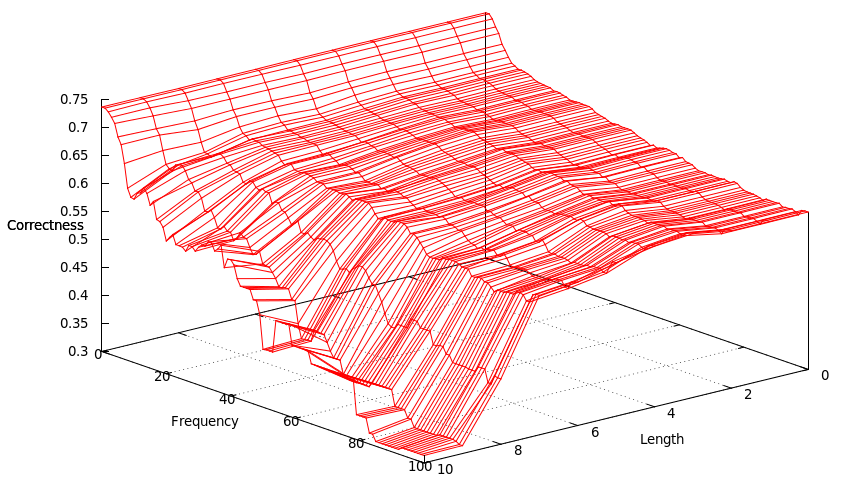
\includegraphics[width=140mm]{img/pak-paroubek-params.png}
\caption{Dobór parametrów algorytmu analizy sentymentu}
\label{image:pak-paroubek-parametry}
\end{figure}